% Also note that the "draftcls" or "draftclsnofoot", not "draft", option
% should be used if it is desired that the figures are to be displayed in
% draft mode.
%
\documentclass[12pt,oneside,letterpaper]{memoir}

% preamble.tex -- packages to include
%
% Wisconsin dissertation template
% Copyright (c) 2008 William C. Benton.  All rights reserved.
%
% This program can redistributed and/or modified under the terms
% of the LaTeX Project Public License Distributed from CTAN
% archives in directory macros/latex/base/lppl.txt; either
% version 1 of the License, or (at your option) any later version.
%
% This program includes other software that is licensed under the
% terms of the LPPL and the Perl Artistic License; see README for details.
%
% You, the user, still hold the copyright to any document you produce
% with this software (like your dissertation).

%% You should use natbib
\IfFileExists{natbib.sty}{%
	\usepackage[numbers]{natbib}%
}{}

%% You probably need appendix, if you want appendices
\IfFileExists{appendix.sty}{%
\usepackage{appendix}%
}{}

%% the spacing in memoir is weird, you'll need to use this
\DisemulatePackage{setspace}
\usepackage[onehalfspacing]{setspace}

%% List setup; the ``hanglist`` environment will allow you to have
%% nicely-typeset enumerated lists (i.e. with the numbers hanging in
%% the margins).  You need at least version 2.1 of enumitem.sty.  If
%% you don't have enumitem installed at all, hanglist will just be an
%% alias for enumerate.
\IfFileExists{enumitem.sty}{%
\usepackage[loadonly]{enumitem}[2007/06/30]%
\newlist{hanglist}{enumerate}{1}% 
\setlist[hanglist]{label=\arabic*.}%
\setlist[hanglist,1]{leftmargin=0pt}%
}{%
\newenvironment{hanglist}{\begin{enumerate}}{\end{enumerate}}%
}

%% Comment out any of these that you don't want
\usepackage{amssymb}
\usepackage{amsmath}
\usepackage{amsthm}
%\usepackage{theorem}
\usepackage{hyperref}

\IfFileExists{mathpartir.sty}{%
\usepackage{mathpartir}%
}{}

%%%%% LISTINGS package and setup
\IfFileExists{listings.sty}{%
\usepackage{listings}%
}{}



%% Get rid of ugly borders around PDF hyperlinks (e.g. for cross-references, bib entries, or URLs)
\hypersetup{pdfborder = 0 0 0}

%% You want microtype.
\IfFileExists{microtype.sty}{%
\usepackage[protrusion=true,expansion=true]{microtype}%
}{}

%\pagestyle{thesisdraft}

% Surround parts of graphics with box
\usepackage{boxedminipage}

%% booktabs (thx to Nate Rosenblum for bringing this beautiful package
%% to my attention)
\IfFileExists{booktabs.sty}{%
\usepackage{booktabs}%
}{}

% This is now the recommended way for checking for PDFLaTeX:
\usepackage{ifpdf}

%% Avoid ugly "Type 3" fonts
\usepackage{lmodern}
\usepackage[LY1]{fontenc}

%% Substitute your favorite serif and sans fonts here....
\IfFileExists{tgpagella.sty}{%
% TeX Gyre pagella, like Palatino
\usepackage{tgpagella}%
}{}

\usepackage[LY1]{eulervm}

\ifpdf
\usepackage[pdftex]{graphicx}
\else
\usepackage{graphicx}
\fi

\usepackage{makeidx}
\makeindex

{\theoremstyle{plain}
\newtheorem{thm}{Theorem}[chapter]
\newtheorem{cor}[thm]{Corollary}
\newtheorem{define}[thm]{Definition}
\newtheorem{exmpl}[thm]{Example}
}
{\theoremstyle{remark}
\newtheorem{rmk}[thm]{Remark}
}

\newtheoremstyle{customsty1}
{3pt}%
{3pt}%
{}% --- body font
{}% --- indent amount
{\bfseries}% --- Theorem head font
{:}% --- Punctuation after head
{.5em}% --- space after head
{}% --- theorem head spec (can be left empty, meaning 'normal')

% Define 'newtheorems' that use ``customsty1''
{\theoremstyle{customsty1} 
}


%%% NB: the ``deposit'' chapter- and page- styles should conform to UW
%%% requirements.  If you are producing a pretty version of your
%%% dissertation for web use later, you will certainly want to make
%%% your own chapter and page styles.

\makechapterstyle{deposit}{%
  \renewcommand{\chapterheadstart}{}
  \renewcommand{\printchaptername}{}
  \renewcommand{\chapternamenum}{}
  \renewcommand{\printchapternum}{\parbox{2em}{\MakeLowercase{\Large\scshape\thechapter{}}} }
  \renewcommand{\afterchapternum}{}
  \renewcommand{\printchaptertitle}[1]{%
  \raggedright\Large\scshape\MakeLowercase{##1}}
  \renewcommand{\afterchaptertitle}{%
  \vskip\onelineskip \hrule\vskip\onelineskip}
}

\makepagestyle{deposit}
 
\makeatletter
 
\renewcommand{\chaptermark}[1]{\markboth{#1}{}}
\renewcommand{\sectionmark}[1]{\markboth{#1}{}}
 
\makeevenfoot{deposit}{}{}{}
\makeoddfoot{deposit}{}{}{}
\makeevenhead{deposit}{\thepage}{}{}
\makeoddhead{deposit}{}{}{\thepage}
\makeatother

%%% set up page numbering for chapter pages to satisfy UW requirements
%%% NB: You will want to delete until the ``SNIP'' mark if you are
%%% making a ``nice'' copy
\copypagestyle{chapter}{plain}
\makeoddfoot{chapter}{}{}{}
\makeevenhead{chapter}{\thepage}{}{}
\makeoddhead{chapter}{}{}{\thepage}
%%% SNIP

%%% bib nonsense
\makeatletter
\newenvironment{wb-bib}[1]{%
  \chapter*{references}
\ifnobibintoc\else 
\phantomsection 
\addcontentsline{toc}{chapter}{References} 
\fi 
\prebibhook
  \begin{bibitemlist}{#1}}{\end{bibitemlist}\postbibhook}

\AtBeginDocument{%
  \@ifpackageloaded{natbib}{% natbib is loaded
    \addtodef{\endthebibliography}{}{\vskip-\lastskip\postbibhook}
    \@ifpackagewith{natbib}{sectionbib}{% with sectionbib option
      \renewcommand{\bibsection}{\@memb@bsec}}%
      {\renewcommand{\bibsection}{\@memb@bchap}}}%
  {}
  \@ifpackagewith{chapterbib}{sectionbib}{%
    \renewcommand{\sectionbib}[2]{}
    \renewcommand{\bibsection}{\@memb@bsec}}{}
}


\newcounter {tocpage}
\newcounter {lofpage}
\newcounter {lotpage}
\newcounter {listofheading}

\newcommand\@thesistitlemedskip{0.2in}
\newcommand\@thesistitlebigskip{0.6in}
\newcommand{\degree}[1]{\gdef\@degree{#1}}
\newcommand{\project}{\gdef\@doctype{A masters project report}}
\newcommand{\prelim}{\gdef\@doctype{A preliminary report}}
\newcommand{\thesis}{\gdef\@doctype{A thesis}}
\newcommand{\dissertation}{\gdef\@doctype{A dissertation}}
\newcommand{\department}[1]{\gdef\@department{(#1)}}

\newenvironment{titlepage}
 {\@restonecolfalse\if@twocolumn\@restonecoltrue\onecolumn
  \else \newpage \fi \thispagestyle{empty}
% \c@page\z@ -- deleted: count title page in thesis
}{\if@restonecol\twocolumn \else \newpage \fi}

\gdef\@degree{Master of Science}    %Default is PhD
\gdef\@doctype{A thesis}         %Default is dissertation

\gdef\@department{(Electrical Engineering)} % Default is Electical Engineering
\gdef\@defensedate{01/01/2100}% Default is a long time from now.

\renewcommand{\maketitle}{%
  \begin{titlepage}
%-----------------------------------------------------------------------------
% -- The thesis office doesn't like thanks on title page.  Put it in
% -- the acknowledgments.  This is here so you don't have to change
% -- your titlepage when converting from report style. -> from Purdue, but I
%        left it here since it seems compatible with UW-Madison, Eric
%-----------------------------------------------------------------------------
    \def\thanks##1{\typeout{Warning: `thanks' deleted from thesis titlepage.}}
    \let\footnotesize\small \let\footnoterule\relax \setcounter{page}{1}
    \begin{center}
      {\textbf{\expandafter\expandafter{\@title}}} \\[\@thesistitlebigskip]
       by \\[\@thesistitlemedskip]
      \@author \\[\@thesistitlebigskip]
      \@doctype\ submitted in partial fulfillment of \\
      the requirements for the degree of\\[\@thesistitlebigskip]
      \@degree \\[\@thesistitlemedskip]
      \@department \\[\@thesistitlebigskip]
      at the \\[\@thesistitlemedskip]
      UNIVERSITY OF WISCONSIN--MADISON\\[\@thesistitlemedskip]
      \@date
    \end{center}
  \end{titlepage}
  \setcounter{footnote}{0}
  \setcounter{page}{1} %title page is NOT counted
  \let\maketitle\relax \let\degree\relax \let\project\relax \let\prelim\relax
  \let\department\relax
  \gdef\@thanks{}\gdef\@degree{}\gdef\@doctype{}
  \gdef\@department{}
  %\gdef\@author{}\gdef\@title{}
}

%=============================================================================
% ABSTRACT
%=============================================================================
% The abstract should begin with two single-spaced lines describing
% the author and title in a standard format.  After these lines comes
% the standard abstract.
%=============================================================================
\def\abstract{
  \chapter*{Abstract}
  \addcontentsline{toc}{chapter}{Abstract}
  \relax\markboth{Abstract}{Abstract}}
\def\endabstract{\par\newpage}


%=============================================================================
% ACKNOWLEDGMENTS
%=============================================================================
% The acknowledgments environment must do the following:
% - start a new page with ACKNOWLEDGMENTS centered two inches from the top
%=============================================================================
\def\acks{
  \chapter*{Acknowledgments}
}
\def\endacks{\par\newpage}


\makeatother


\usepackage{hyperref}

\usepackage{ifpdf}

\ifpdf
   \usepackage[pdftex]{graphicx}
  % declare the path(s) where your graphic files are
  \graphicspath{{../pdf/}{../jpeg/}}
  % and their extensions so you won't have to specify these with
  % every instance of \includegraphics
   \DeclareGraphicsExtensions{.pdf,.jpeg,.png}
  \hypersetup{pdfborder = 0 0 0}
\else
  % or other class option (dvipsone, dvipdf, if not using dvips). graphicx
  % will default to the driver specified in the system graphics.cfg if no
  % driver is specified.
   \usepackage[dvips]{graphicx}
  % declare the path(s) where your graphic files are
   \graphicspath{{../eps/}}
  % and their extensions so you won't have to specify these with
  % every instance of \includegraphics
   \DeclareGraphicsExtensions{.eps}
\fi

\graphicspath{ {MS_figs/} }

\usepackage{array}


\usepackage{mdwmath}
\usepackage{mdwtab}

\usepackage{eqparbox}

\usepackage[caption=false,font=footnotesize]{subfig}

\usepackage{url}

\usepackage{eulervm}


\hyphenation{op-tical net-works semi-conduc-tor}


\begin{document}
%
% paper title
% can use linebreaks \\ within to get better formatting as desired
\title{Hardware Design of a Integrated Modular Motor Drive (IMMD)}
\author{Adam Shea}


% make the title area
\maketitle
\clearpage

\input{MS_parts/abstract.tex}

\clearpage
\tableofcontents

%\clearpage
%\listoftables

\clearpage
\listoffigures

\clearpage

\chapter{Introduction}
The increasing proliferation and maturation of electric drive technologies has
caused drive system-level integration to become a high priority in a variety
of application areas including electric propulsion, aerospace, white goods,
and down-hole drilling.
Tight integration of motor and drive electronics
offers attractive properties including reduced overall system volume,
reduction of high-current cabling, reduced radiated EMI, simplified cooling
arrangements, and appealing fault tolerance opportunities.

However, physical integration of electric machines and drives presents many
challenges.
In order to integrate the controls and power electronics into the
machine housing, the power electronics must be designed to operate reliably in
elevated vibration and thermal environments that fall outside of standard
ranges for industrial-grade components.
Further complicating the
challenges, customers for integrated drives typically expect the drive
electronics to meet or exceed the lifetime of the machine, requiring very high
reliability in demanding environments.

Early generations of integrated motor drives have typically used conventional
three-phase induction or PM synchronous machines combined with standard
voltage-source 6-switch bridge inverters to excite the machine.
In many of these units, the drive is housed in its own enclosure which, in
turn, is mounted on the side or end of the machine.
More aggressive concepts for integrated machine drives have been proposed that
approach more closely the ultimate objective of mounting the complete drive
inside the same enclosure as the machine, but commercialization of these
advanced integrated drive architectures has been limited to date.

One of these advanced concepts that has been proposed in the literature is the
integrated modular motor drive (IMMD) .
As illustrated in Fig. \ref{figCPESIMMD}, this
concept segments the stator into individual pole pieces, each encircled by a
concentrated winding that is excited by its own dedicated electronics unit
that includes both the necessary power electronics and controls to form a
complete pole-drive unit.
The IMMD is completed by interconnecting a number
of these pole-drive units to form an annulus around the rotor.
Appealing features of this IMMD concept emerge from its modularity, offering
opportunities for improved manufacturability, enhanced fault tolerance and
redundancy, and simplified repair/replacement of the pole-drive units.

\section{Motivation}

\subsection{Reliability and Redundancy}
As electric drive systems move into many power and actuation applications
previously handled by mechanical and hydraulic systems, reliability and
redundancy becomes an important consideration for an electric drive.

In aerospace systems, a typical fault mitigation method is to use parallel
actuators which are torque summed in order that a failed actuator does not
cause system failure \cite{Annaz09}.
While this method is well understood and robust, it requires significant extra
weight, volume, and cost over a single actuator able to perform the same task.

Argile et al. \cite{Argile08} described a Markov model method for describing
converter faults and calculating the total MTTF for a fault-tolerant converter
model which is able to continue operation even in the face of lost power
conversion components.
This paper shows clearly both the difficulties posed by the increased failure
rates caused by increasing component counts and the opportunities afforded by
fault tolerance when repair is possible.


\subsection{EMI Containment}
As electric drives spread into automotive and residential areas at high
powers, EMI mitigation becomes a major design challenge.



\section{Previous Research}
Previous research into integrated modular motor drives can be split into three
categories.
\subsection{System Level Designs and Integrated Converters}
The first category, system-level research includes investigations into
controlling high phase-order machines and fault tolerant drives to achieve
continued system operation in the presence of machine and drive component
failures.

The first of these investigations was carried out with a load commutated
thyristor based inverter and a 6-phase induction machine.
In his research \cite{Jahns78} T. M. Jahns achieved full torque operation of a faulted
machine with only minimal increase in machine and drive losses though the
modification of applied voltage magnitude and frequency to the remaining
healthy phases.

More recent related research has been undertaken at WEMPEC in the area of
modular converter integration.

Recently Nate Brown and others \cite{Brown07a} have demonstrated a fully
modular machine consisting of tooth-wound SMC pole pieces coupled to a
modularized inverter.
\begin{figure}[htbp]
\centering
\label{figCPESIMMD}
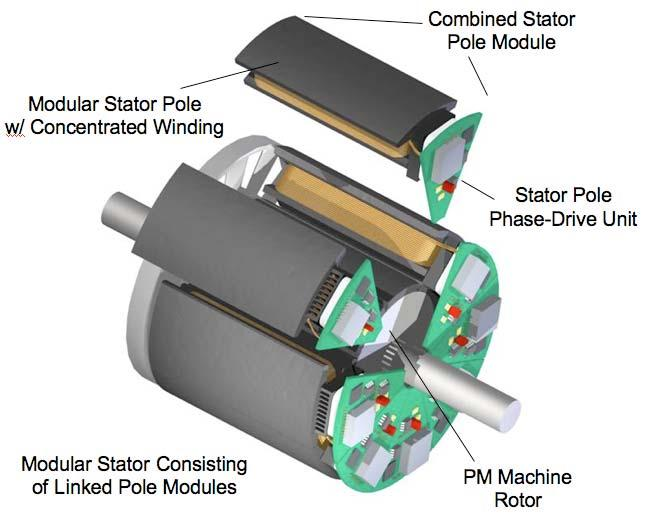
\includegraphics[width=5in]{IMMD3k}
\caption{Rendered views of 5-phase SMC modular motor drive.}
\end{figure}
The entire machine and drive are air cooled by drawing air first through the
inverter poles then through the machine airgap and slots.
The controls on this machine however are still fully centralized.

This modular inverter also demonstrated the difficulties in modular drive
interconnect as its phase and power connections developed intermittent faults
after a relatively short operating life.


\subsection{Machine Design}
The next category and a vital component of any motor control work is the
design of the electric machine itself.

In order to allow easy redundancy and increased flexibility of operating with
multiple phase configurations, this works focuses on a 6-phase machine with a
60 degree phase spacing.
A dual winding 12 slot, 10 pole dual-layer design was chosen due to the
highly isolated and contained flux paths \cite{Bianchi05}.
This design allows for machine characterization and testing using standard 3
phase converters which greatly helps both in model design and system
debugging.


\subsection{Current Sensing}
Accurate current sensing is a vital component of high-performance motor
controls.  Often this is accomplished through the use of transformer-based
hall-effect sensors.  Sadly, for an integrated application these sensors are
both highly temperature sensitive and too large.

A much more compact current sensing method involves the use of free-space
magnetic field sensors in fixed position relative to a current carrying
conductor.
This approach allows both small-size and high bandwidth as current sensor core
materials do not come into play.
In \cite{Schneider10} GMR sensors are used as they allow for extremely large
bandwidth (into the MHz range).
These sensors are however unipolar and biasing magnet requirements offset some
of the thermal stability gains.



\chapter{Abstract Design}

\section{Control Topology}


\subsection{Non-synchronized PWM}
While control states may be managed between modular drive processors with only
moderate difficulty, the classical assumption that all PWM carriers are
synchronized presents significant difficulty as a delay of only a few
microseconds represents a significant phase delay.
Thankfully, at normal carrier to fundamental ratios, the phase of the PWM
carrier is unimportant to a first order as the machine inductance filters out
the high frequency switching components.
Quartz crystal-based main oscillators are quite stable and allow frequency
tolerance below 100ppm without any special calibration.
For a 20kHz PWM system, the beat frequency between PWM carriers will be at a
frequency of 2Hz.
This beat frequency will manifest as a peaking of the $\frac{dV}{dt}$ applied
to the machine windings relative to the frame every 0.5s or longer depending
on the specific spread of oscillator frequencies.
While this phenomenon has little effect on the control of the machine, the
effects on bearing currents and insulation lifetime have not been investigated.

\subsection{Fault Management}
A detailed consideration of fault management has been reserved for future work, but 

\section{DC-Link Design}
DC-link design is a topic that is often overlooked in converter design.
Usually it is relegated to rules-of-thumb which are often based on sound
reasoning, but typically end up being used in situations where the assumptions
they are based on do not hold.

The first of these rules is to size DC-Link capacitors based on a certain
capacity per Watt of converter power rating.
This rule is extremely easy to apply, but is typically based on the assumption
of DC-Link currents being dominated by the 120Hz or 180Hz current ripple of a
single-phase or 6-pulse diode rectifier.
This rule also is specific to one voltage level as the ripple current and thus
capacitance requirement is decreased as the inverse of the DC-link voltage.
If not driven by controls requirements on DC-link voltage variation, this rule
also assumes specific current handling capabilities of the capacitor
(Typically electrolytic).

The next common rule is to design based on an allowed voltage ripple.
This rule is significantly more robust than the converter-power based rule
above as it takes into account varying ripple current conditions.
This rule is also often dictated by the controls design as control accuracy
will suffer if the DC-Link voltage variation is not decoupled.

A final rule of thumb is to size the DC-link capacitance to be thermally rated
for a ripple current that is a given fraction of the converter's rated output
current (typically one third for common 3-phase converters).
This is a very robust rule in terms of managing component lifetime, but may
cause excess DC-Link voltage ripple if polymer film-based capacitors are used
due to their excellent current handling capability even at low capacitance
ratings.

These three rules all encapsulate both their driving assumptions the two
actual drivers of DC-link design.

First, whatever design is chosen must be capable of handling ripple-related
thermal loads.
This is a function of both dielectric heating effects and joule
losses in capacitors and inductors.
As capacitor technology advances with
improvements in film capacitors and upcoming dielectric materials such as
glass, designs based on thermal capability will become more necessary.

Second, a DC-link structure is at its core an impedance matching component
which must present a low impedance to the power converter's switching pole
at the switching frequency and higher, must present a low impedance at twice
the power frequency due to reactive power handling requirements, and must
present a high impedance at DC in order to ensure that bulk power flow comes
from the power source.

While this is typically handled with bulk capacitance for standard VSI-based
designs, the size and temperature constraints of the integrated modular motor
drive require a more creative hybrid approach.
An interesting aside is that resonant-link converters fully exploit this
requirement to reduce switching losses and reactive component size.

\subsection{Interconnect Design}
For the integrated modular motor drive, we cannot tolerate the low temperature
ratings of electrolytic capacitors.
Because of this limitation, the total bulk capacitance available is much lower
than would typically be used in a converter of this size.
Furthermore, due to the distributed nature of the converter, reactive power
currents must be passed through the DC-link structure to other modules before
returning to the machine.
In order to maintain an effective low impedance at the power frequency for
reactive power while shielding these currents from the power source, a
star-and-ring topology was chosen as described in previous work on IMMD power
electronics.

While this ring-and-star approach is very effective at handling
power-frequency harmonics, it does not keep a stiff DC-link at the switching
frequency and higher.
In order to accomplish this, I chose a frequency-splitting technique similar
to what is used in high performance logic decoupling.
To this end, the DC-link capacitance is split into three parts on each module:
A bulk polyproylene film capacitor, a pair of multilayer ceramic capacitors,
and an integrated PCB capacitor.


\subsection{Capacitor Sizing}
Capacitor sizing was based entirely on current handling capability and size
constraints.
As power-frequency components are being primarily handled by the DC-Link
interconnect we require little capacitance to manage reactive power flow.
For the bulk DC-link capacitance, a 700V 20$\mu F$ film capacitor from TDK was
chosen as it can handle nearly the entire ripple current of a phase at rated
load.
This capacitor will be absorbing the kHz range ripple from the converter
switching.
The ceramic capacitors were chosen for high-voltage, low-inductance, and low
dielectric loss.
As these capacitors are placed directly on the DC terminals of the power
modules, they will be handling the MHz range power frequencies caused by
switching edges.
Finally, the PCB itself was designed with nearly uniterrupted power planes
which provided each board with 1nF of somewhat lossy capacitance at very low
inductance which ensured that >10MHz ripple would not be injected into the
other capacitors.

This multi-layer design allowed for low impedance with reduced overall
capacitor size as is shown in the results section.


\section{Peak Ratings}
Electric machine and drive system ratings are influenced by a variety of
factors.
While continuous ratings for rated operating conditions are well defined and
easily modeled and tested, peak ratings are dependent on definitions.
The determination of peak ratings is further complicated by marketing
influences in that a large "peak power" number is an easily quoted figure of
merit even if it has little real-world backing.

The peak rating of an electric drive system is driven by a number of factors
depending on the peak time required.
For peak times on the order of one electrical cycle, the power limit is driven
by the saturation current allowed by the power switches and the
demagnetization limit of the permanent magnets in the electric machine.
Both of these limits are effected by the starting temperature of the
electrical drive system, but are largely independent of other thermal effects
as the peak time is too short.

For the FreedomCar/USDrive specification, peak power rating is defined as an
83\% overload for 18 seconds.
This overload time is of the same order as machine thermal time constants.
From a converter sizing standpoint, this overload rating requires that the
power switches are capable of handling the full overload power as they have
sub-second thermal time consents.
The remainder of the converter design however only needs to be rated to the
continuous load as capacitor and interconnect thermal time constants are
measured in minutes or longer.
The cooling system for the power converter must be able to handle
approximately the same overload as the machine as the extra cooling load from
the power semiconductors will increase in proportion to output power.
Finally, sensing must be able to accommodate the full overload if control is to
be maintained during overloaded conditions.


\chapter{Detailed Design}
In this chapter I describe in detail the design of the modular motor drive
modules and system.
In the sections that follow, the specific design choices and design drivers
are outlined and schematic sections are presented.
Overall drive component schematics and PCB layouts are contained in Appendix
\ref{appCAD}.

\section{Mechanical Layout}
An important part of any integrated converter design is the mechanical layout
and packaging or as some would say: "multiphysics integration".
For this integrated modular drive design, the converter and all its controls
will be mounted on the end of a 6-phase machine designed at 1/3 scale but full
diameter for the FreedomCar/USDrive specification.

In order to shield the drive from EMI and fringing fields from the machine,
the drive is mounted on a stainless steel baseplate of the same footprint as
the stator.
The drive consists of six phase drive modules which mount over the
corresponding two stator tooth section of the machine.
Each module is one sixth of the stator circumference.
In order to allow easy fabrication each module consists of two printed circuit
boards with bolt together interconnects which both allows for low-resistance
connection for high-current paths and the ability to quickly change out
damaged modules in case of faults.

Cooling is designed to be possible with either water or air.
In this case water cooling is used as the machine is already cooled with a
water jacket.
The drive modules plumbed in series, upstream of the machine cooling water
jacket.

\section{Gate Drivers}
Gate drive design for a tightly integrated motor drive is primarily driven by
a need for small size and high output current.
In this design, the DC-Link voltage is less than 400V which allows the use of
commercial integrated bootstrap gate driver chips.

The FAN7390 integrated bootstrap gate driver was chosen as it supplies peak
switching currents of more than 4 amps and handles undervoltage lockouts to
ensure safe startup.
This device is supplied in an 8 pin SOIC package and requires an external
diode and bootstrap capacitor for high side supply.
The temperature rating is for less than 150C junction temperature which
requires less than 300mW of power dissipation in order to allow full
temperature range operation in this design.
Gate turn on and turn off is controlled through the use of a 10 Ohm turn on
resistor with a turn off diode to help guard against shoot-through and ensure
that Miller current injection cannot turn on the IGBTs.

Power stage desaturation is measured on the low side by use of a diode clamped
connection to the switching node tied to the 15V gate supply.
This signal is then buffered by a P-channel MOSFET before being fed into a
digital input to the DSP.
In the case of lower switch desaturation, this input will remain low which
indicates to the software that a fault has occurred.
In the case of high side desaturation, the fault can only be detected if the
switching node voltage drops below 15V.
This sensor can also detect shorted power switches within one switching cycle
due to state mismatch with the gate drive commands.

\section{Power Module}
While the power rating for this design is only 18kW, the system design was
implemented with higher power ratings in mind.
To this end, a small PCB was made to carry two discrete 600V IGBT-diode
CoPacks, an RTC temperature sensor and a phase current busbar.
This module mimics standard half-bridge IGBT modules from suppliers like
Powerex and Semikron at a smaller footprint and power rating more in line with
the design goals of this system.
The power module attaches to the control board by way of two bolt-down
connections for the DC-Link and an 8 pin 100 mil header for gate connections
and temperature sensing.
The phase conductor busbar is used as part of the current sensing system
described in the next section.
This module is then strapped to the heatsink using a fiberglass clamp to cool
the IGBTs.
The design here allows for either air or water cooling though water cooling
with a low cost video card water block was implemented during construction.

\section{Current Sensing}
Current sensing in this modular design was primarily driven by availability
and ease of integration.
While closed-loop sensors are most common for high performance motor drives,
their requirement of encircling the phase conductor to be sensed meant that
integration and easily disassembly would be difficult.
Giant Magnetoresistive (GMR) sensors were also considered as they provide very
small packages with excellent frequency response and dynamic range.
GMR sensors however are more immature in the current sensing space and the
unipolar nature of the sensor means that significant support is needed in
terms of biasing and signal processing.
The lack of a polished current sensing solution based on GMRs ruled them out
of this design.

The current sensing design for the integrated modular motor drive was finally
chosen to be an open-loop hall effect field sensor.
The FHS 40-P device from LEM is a small SOIC-8 packaged device with minimal
signal conditioning circuitry which is both low-cost and readily available.
In order to use this device, it must be mounted on an area of PCB with an open
aperture in the ground plane beneath it as is shown in figure
\ref{figHallPCB}.
The current in a conductor mounted a fixed distance away is then sensed by
measuring the magnetic field impinging on the sensor.

The spacing between the sensor and current carrying conductor is managed by
the bolt-together standoffs between the controller board and the power
semiconductor module.

Using a free-space field sensor in an application tightly integrated with an
electric machine presents special challenges which were only exacerbated by
the rotor in this machine being three times the length of the stator.
In order to ensure current sensing was not contaminated by offsets and noise
from the machine below, the baseplate was chosen of a semi-ferromagnetic
material (304 Stainless Steel) in order to shield low-frequency magnetic
fields from the sensor.
The copper faceplate of the water block directly below the power semiconductor
module adds a further layer of shielding, using eddy currents to block higher
frequency interfering fields from the sensor.

\section{DSP}

\section{Communications}


\chapter{Discussion}

\section{Hardware Performance}

\section{Scaling}


\chapter{Conclusions}

\section{Future Work}

\subsection{Multi-phase IMMD}

\subsection{EMI analysis}

\subsection{Control Development}

\subsection{High-temperature Testing}


\bibliography{bib}


% that's all folks
\end{document}


